% 本文件作为当前原理章节的入口；原有 content/2principle.tex 保持不变。
\section{实验原理}

%  本节参考课程讲义《密码分析的自动化搜索模型》中关于非零位置点集的建模方法。\footnote{胡凯：《密码分析的自动化搜索模型》，2026年10月20日，Part 1，第10--27页；线性掩码传播参见第45--46页。}讲义以三位S盒$\chi_3$说明方法，本实验则按实验指导书使用四位CipherFour S盒；两者的建模步骤相同，但点的维数、具体系数和实验结果需要分别确定。

\subsection{DDT与LAT}
根据课程所学的差分分析和线性分析，这里简单复述一下S盒的差分分布表(DDT)和线性分布表(LAT)。

\subsubsection{DDT}
对于一个$m \times n$的S盒，即映射$S:\mathbb{F}_2^m \to \mathbb{F}_2^n$，记满足输入差分$\alpha$、输出差分$\beta$的输入集合为
$$
IN_S(\alpha ,\beta) = \{X \in \mathbb{F}_2^m :S(X) \oplus S(X \oplus \alpha) = \beta\}.
$$
DDT中的表项为该集合的元素个数，即
$$
\operatorname{DDT}[\alpha][\beta] = \# IN_S(\alpha,\beta).
$$

\subsubsection{LAT}

对于同一个$m \times n$的S盒，LAT是一个$2^m \times 2^n$的表，其中第$\alpha$行第$\beta$列的表项为
$$
\operatorname{LAT}[\alpha][\beta]
=\#\{x\in\mathbb{F}_2^m\mid \alpha\cdot x\oplus\beta\cdot S(x)=0\}-2^{m-1}.
$$
这里$\cdot$表示模$2$内积。该表项是输入、输出掩码为$\alpha,\beta$时，使线性表达式$\alpha\cdot x\oplus\beta\cdot S(x)$等于$0$的输入个数与$2^{m-1}$的差，其值与输入总数$2^m$的比值恰好为线性近似的偏差：
$$
\epsilon(\alpha,\beta)
=\Pr[\alpha\cdot x=\beta\cdot S(x)]-\frac{1}{2}
=\frac{\operatorname{LAT}[\alpha][\beta]}{2^m}.
$$


对于有限的点集,我们可以列出所有的点，那也就是说，它的边界肯定是直线
\subsection{MILP}

搜索差分路线是一件比较困难的事情,在算法功底扎实的情况下，我们确实可以通过dfs或者动态规划来求解问题
,不过在纯人工的角度下来说，这个还是比较困难的，毕竟不同的问题我们就需要设计不同的算法,虽然说有AI可以解决，但是本质上还是特题特解

所以说如果我们有一个自动化的工具，那无疑是更好的，自动化工具的本质其实就是把编程问题抽象成数学问题
.因为本质上就是优化问题，那只要我们能把问题数学建模，数学上的优化方法要远比我们编程的算法要普适得多

在我们得到了DDT和LAT之后,我们希望把他里面的东西变成数学对象,以致于我们可以用线性规划之类的数学优化方法来求解
,在这里我们可以用MILP(Mixed Integer Linear Programming)来建模,也就是混合整数线性规划,形式如下
\[
\begin{aligned}
\min \quad & c^T x+d^T y\\
\text{s.t.}\quad & Ax+By\leq b\\
& x\in\mathbb R^n\\
& y\in\mathbb Z^m
\end{aligned}
\]

目标函数（Objective Function）：\(c^Tx+d^Ty\)，要求最大化或最小化。

约束条件（Constraints）：\(Ax+By\leq b\)，必须是线性的，也可以包含线性等式

连续变量：\(x\in\mathbb R^n\)。

整数变量：\(y\in\mathbb Z^m\)，其中二进制变量 \(y_i\in\{0,1\}\) 是常见的特殊情况

MILP 的核心就是：目标函数和约束都是线性的，但部分或全部变量必须取整数

不过在密码学中连续的变量其实很少出现，其实这里是ILP,也就是Integer Linear Programming

那这个问题我们其实在组合学图论这门课程中遇到过
\begin{figure}[H]
    \centering
    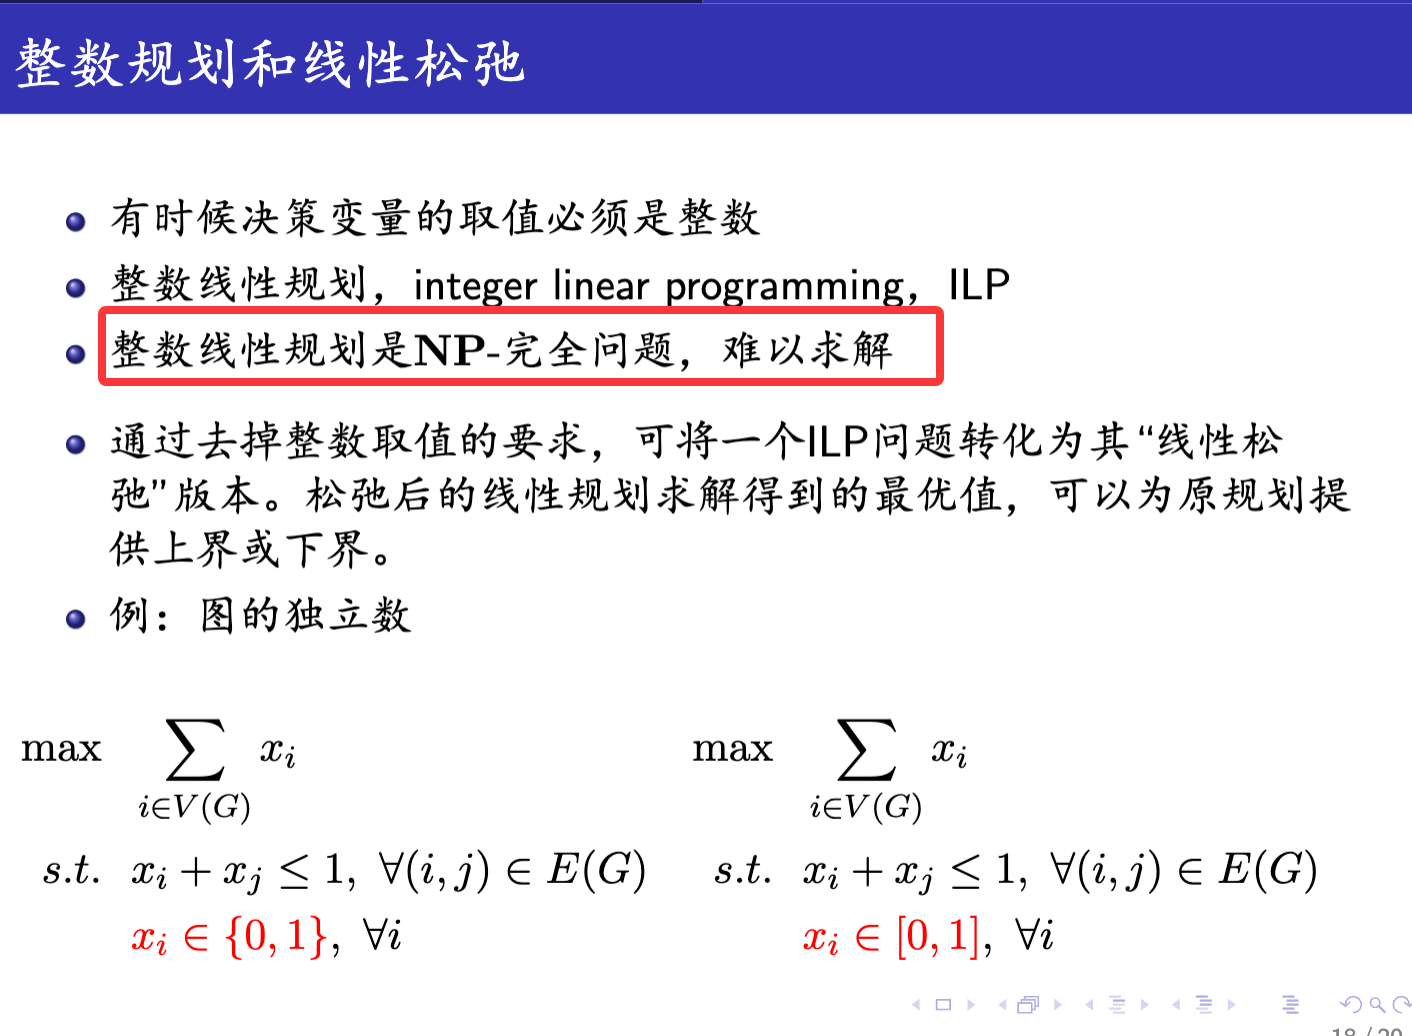
\includegraphics[width=0.8\textwidth]{figures/ILP.png}
\end{figure}

那你会发现这是一个NPC问题,是没有多项式时间算法的(至少现在)

那我们规约成NPC问题真的合适吗?关键是S盒的路线本来就是指数级别的,那即使你用dfs或者动态规划，他其实也是指数复杂度的

所以说既然如此我们不如用MILP来建模,因为MILP有很多现成的求解器,比如gurobi,它是一个非常强大的求解器,可以在很短的时间内求解大规模的MILP问题


\subsection{点集的刻画}
目标函数肯定是明确的，就是最优的路线

关键是约束条件怎么写,在我们得到DDT和LAT之后,那怎么判定一条路线能不能走通呢？

DDT就统计了所有的输入差分和输出差分的组合,如果这个组合在DDT中是大于0的,那就说明是可以走的通的，无非就是概率大小的事

LAT考虑的是偏差，那有正有负，只要不等于0，就说明有机会

所以说我们不妨记
\[
M[b,a]=\frac{\operatorname{DDT}[a][b]}{16}
\]
这就表示从输入差分$a$到输出差分$b$的概率,只要这个概率大于0，那就是可达的

那我们的差分路线本质上就是在这些可达的地方不断移动，这个所谓的\(M[b,a]\)就很像平面直角坐标系里的一个点

那我们把这些可达的点\[M[b,a] \neq 0\]构成一个点集,记作$supp(M)$
\[
V_M = \{(a,b) \mid (a,b) \in \text{supp}(M)\}
\]

那这个点集就是差分传播的研究对象
线性近似路线也是一样的，我们用相关度来表示
\[
C[b,a]=\frac{\operatorname{LAT}[a][b]}{8}
\]
那我们把这些可达的点\[C[b,a] \neq 0\]构成一个点集,记作$supp(C)$
\[
V_C = \{(a,b) \mid (a,b) \in \text{supp}(C)\}
\]

那你说建模很简单啊，约束关系就写$v \in V,v \notin V$不就行了

对于人来说这个属不属于当然简单，不过它并不是一个线性运算啊

这个属于关系没办法写成加减乘除的形式，在编程里判断属于关系也是比普通的运算复杂的，虽然说python有in运算，不过那也只是封装了而已

那你像C语言中我们判断属于关系，朴素的情况下就是遍历数组的所有元素，判断是否相等

所以说这个属于关系和线性是搭不上边的

进一步说我们考虑一个例子
\[
(a,b)\in V
\]
例如：
\[
S=\{(1,2),(1,3),(2,1)\}
\]

约束实际上等价于
\[
(a=1\land b=2)
\lor
(a=1\land b=3)
\lor
(a=2\land b=1)
\]

那属于的本质其实可以理解为析取的运算，但是这个显然不是线性的

那所以说关键就是把点集建模成数学变量，让它能用线性的式子去刻画属于关系
\subsection{S盒传播的建模}
\label{subsec:lab4-modeling-conventions}

我们可以随便建模，但是怎么验证我们约束的正确性呢？

一个比较耍赖的逻辑是，求解器求出来的解，肯定是满足约束的

试想一下，如果我们直接把目标函数设成常数会得到什么？
\begin{equation}
\begin{aligned}
\min\quad &0\\
\text{s.t.}\quad & ...
\end{aligned}
\end{equation}
如果目标函数是常数，那么所有满足约束条件的解都是最优解

也就是说我们的第一步是，找到一组约束和变量，使得他们的解是点集$V$,那这就能说明我们建模是正确的

在验证单个S盒的传播约束后，要搜索整条差分或线性路线，还需按轮复制这些约束，加入轮间置换连接关系与局部概率或相关度权重，再设置相应的优化目标。

我们先把坐标写成二进制的形式

Cipherfour使用$4\times4$ 的S盒。对于$(a,b)$，按大端序展开
\[
(a,b)\rightarrow (a_3,a_2,a_1,a_0,b_3,b_2,b_1,b_0)\in\{0,1\}^{8},
\]
这个向量我们记作$\text{bits}(a,b)$
那你说本来就两个变量，为什么要弄成8个变量呢，额这其实另有考量，我们后面再谈

\subsection{one-hot法}
\label{subsec:lab4-one-hot}

\paragraph{基本原理}

一个最直接的想法就是，我们直接就给所有点一个变量，集合的属于其实就是0,1关系嘛，0就是不属于，1就是属于

所以说我们给每个点一个0,1变量,记作$\lambda_{(a,b)}$，如果点$(a,b)$属于点集,那么$\lambda_{(a,b)}=1$，否则$\lambda_{(a,b)}=0$

那你求点集里的点，其实就是\(\lambda_{(a,b)}=1\),然后其他都是0

所以约束条件就出来了，\[
\sum_{(a,b)\in V}\lambda_{(a,b)}=1,
\]

\paragraph{数学建模}
\begin{equation}
\begin{aligned}
\min\quad &0\\
\text{s.t.}\quad
&\sum_{(a,b)\in V}\lambda_{(a,b)}=1\\
&x=\sum_{(a,b)\in V}\lambda_{(a,b)}\operatorname{bits}(a,b)\\
&\lambda_{(a,b)}\in\{0,1\},\forall(a,b)\in V
\end{aligned}
\label{eq:lab4-one-hot-model}
\end{equation}


\paragraph{正确性分析}

对于模型的任意可行解，由 $\lambda_{(a,b)}\in\{0,1\}$ 以及
\[
\sum_{(a,b)\in V}\lambda_{(a,b)}=1
\]
可知，存在唯一的 $(a^*,b^*)\in V$，使得
$\lambda_{(a^*,b^*)}=1$，其余选择变量均为 $0$

将其代入坐标约束
\[
x_j=\sum_{(a,b)\in V}
\operatorname{bits}(a,b)_j\lambda_{(a,b)}
\]
可得
\[
x_j=\operatorname{bits}(a^*,b^*)_j,
\quad j=0,1,\ldots,7.
\]
因此，$x=\operatorname{bits}(a^*,b^*)$，即 $x$ 对应于 $V$ 中的点，不会有不可达的点

反过来，任取 $(a,b)\in V$，令
\[
x=\operatorname{bits}(a,b),\qquad
\lambda_{(a,b)}=1,
\]
其余选择变量均为 $0$，则显然满足模型中的全部约束

\paragraph{用于差分与线性传播}

差分建模时取$V=V_{\mathrm D}$，每个选择变量对应一个DDT非零位置；线性建模时取$V=V_{\mathrm L}$，每个选择变量对应一个LAT非零位置。也可以直接用$(a,b)$给选择变量编号，记作$\lambda_{(a,b)}$，从而与原表中的位置一一对应。两类模型分别建立各自的选择变量，坐标约束形式保持一致；全零点的选择变量也需要保留，以表示未活跃S盒。表项的具体数值不作为这里的优化目标，枚举结果应覆盖全部可达点。

\subsection{逐点排除法}
\label{subsec:lab4-point-exclusion}

\paragraph{基本原理}

简单来说就是正难则反，我们如果能求出点集的补集，那也能刻画出点集

也就是说我们排除掉不可达的点，剩下的就是可达的点了，那怎么排除呢？

我们知道两个点重合就意味他们的距离为0，如果距离大于0，那就意味着两个点不是同一个点，可以用这个特性来排除

那距离首先想到的就是Euclid距离

设不可达点集为
\[
Q=\{0,1\}^{8}\setminus V.
\]
我们
对于任意$q=(q_1,\ldots,q_8)\in Q$
\[
d(x,q)
= \sqrt{\sum_{i=1}^8 (x_i-q_i)^2}
\]
我们知道二进制不管怎么加减无非就是0,1,-1,那么也就是说\((x_i-q_i)^2 = |x_i-q_i|\)

那我们再按$q_i$的值来分的话

如果$q_i=0$,那$|x_i-q_i| = |x_i| = x_i$,

如果$q_i=1$,那$|x_i-q_i| = |x_i - 1| = 1-x_i$,因为$x_i-1 \leq 0$

那么也就是说
\[
d(x,q)
=\sqrt{\sum_{j:q_j=0}x_j+\sum_{j:q_j=1}(1-x_j)}
\]

那我们希望是整数，干脆就不要开根号了，反正没什么区别

那这其实就是Hamming距离

对于任意$q=(q_1,\ldots,q_8)\in Q$，定义$x$与$q$的Hamming距离
\[
d(x,q)
=\sum_{j:q_j=0}x_j+\sum_{j:q_j=1}(1-x_j).
\]

\paragraph{数学建模}
\[
\begin{aligned}
\min\quad &0\\
\text{s.t.}\quad
&\sum_{j:q_j=0}x_j+\sum_{j:q_j=1}(1-x_j)\ge1,
&&q\in Q,\\
&x_j\in\{0,1\},
&&j=1,\ldots,8.
\end{aligned}
\]
也可以进行移项
\[
\sum_{j:q_j=0}x_j-\sum_{j:q_j=1}x_j
\ge1-\sum_{j=1}^{8}q_j,
\qquad q\in Q
\]

例如，输入为$0$、输出为$1$对应的点为$q=0000\,0001$,我们如果要排除它，就可以写成
\[
x_1+x_2+x_3+x_4+x_5+x_6+x_7+(1-x_8)\ge1.
\]


\paragraph{正确性分析}

对于任意不可达点 $q\in Q$，若 $x=q$，则
\[
d(x,q)=\sum_{j:q_j=0}x_j+\sum_{j:q_j=1}(1-x_j)=0,
\]
不满足约束 $d(x,q)\ge1$，所以不可达点都被排除了

反之，若 $x\ne q$，由于 $x,q\in\{0,1\}^8$，
则至少存在一个坐标 $j$ 使得 $x_j\ne q_j$，
因此 $d(x,q)\ge1$，也就是说只排除$q$这一个点

对于任意可达点 $x\in V$，由于 $V$ 与 $Q$ 不相交，
因此对于所有 $q\in Q$，均有 $x\ne q$，
从而满足全部约束，不会有可达点遗漏

反过来，若 $x\notin V$，则根据
$Q=\{0,1\}^8\setminus V$，必有 $x\in Q$。
此时模型中存在针对 $q=x$ 的约束，而
$d(x,q)=0$，与 $d(x,q)\ge1$ 矛盾,所以不会引入任何不可达点。

综上，模型的二进制可行解集合恰好为 $V$，即
\[
\left\{
x\in\{0,1\}^8\;\middle|\;
\sum_{j:q_j=0}x_j+\sum_{j:q_j=1}(1-x_j)\ge1,
\ \forall q\in Q
\right\}=V.
\]

\paragraph{用于差分与线性传播}

差分建模时，将DDT零位置对应的八位向量作为$Q$；线性建模时，将LAT零位置对应的八位向量作为$Q$。两种情况下均只使用原始变量$x$，不需要额外的选择变量。

\subsection{逻辑化简法}
\label{subsec:lab4-logic-minimization}

\paragraph{基本原理}

前面我们通过Hamming距离，为每个不可达点构造一条线性不等式，从而将其排除。

但是这样有一个问题，就是如果不可达点太多，那么需要添加的约束也会非常多

那能不能用一条约束同时排除多个不可达点呢？
\begin{figure}[H]
    \centering
    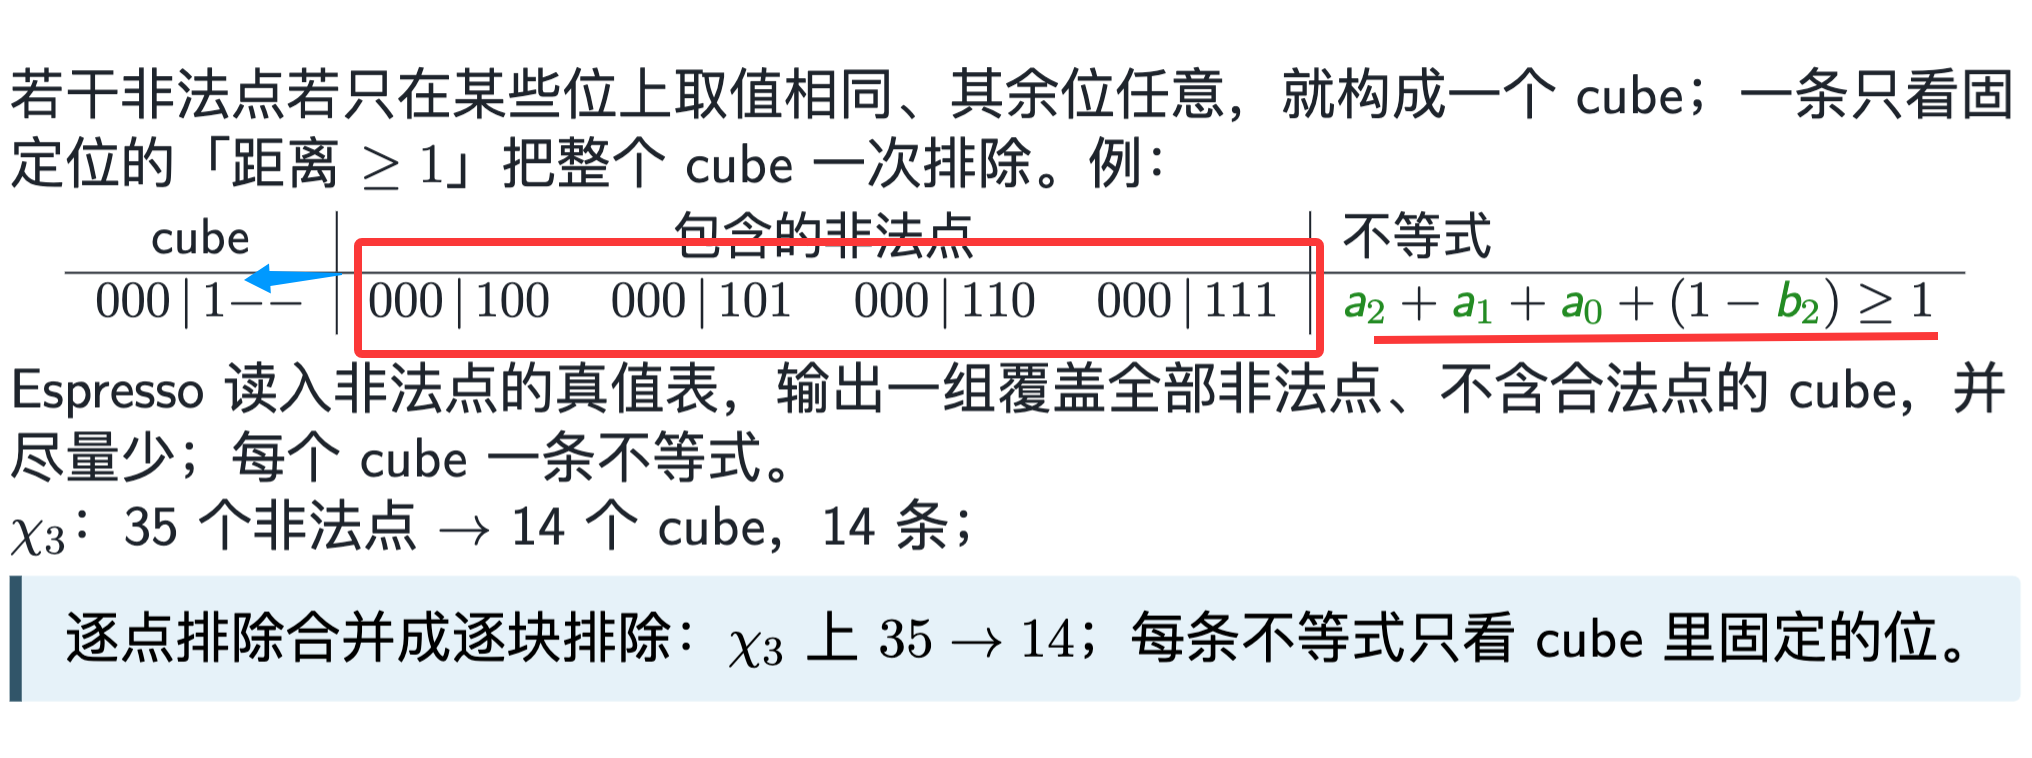
\includegraphics[width=0.8\textwidth]{figures/logic.png}
\end{figure}
就比如课件里这个例子,不可达点的前四位都是0001,那这样我们就可以合并成一个不等式，本来是需要四个的

逻辑化简法将这些点作为布尔函数的取值为$1$的输入，其实就有点像数字逻辑里的卡诺图化简

通过Espresso等工具合并为cube，再对每个cube建立一条排除约束

一条这样的约束可以同时排除该cube覆盖的全部不可达的点


\paragraph{不可达点的布尔表示}


首先，设不可达点集合为
\[
Q=\{0,1\}^{8}\setminus V.
\]

我们定义一个布尔函数
\[
f_{\mathrm{bad}}(x)=
\begin{cases}
1,&x\in Q,\\
0,&x\in V.
\end{cases}
\]

接下来，我们可以把这个函数的真值表交给逻辑化简工具，尝试把多个不可达点合并起来

一般来说，一个cube可以写成
\[
c=(c_1,\ldots,c_8)\in\{0,1,-\}^{8}.
\]

其中$0$和$1$表示对应位置必须取固定值，而$-$表示这一位可以任意取值

为了方便后面构造约束，我们记
\[
I_0(c)=\{j\mid c_j=0\},
\qquad
I_1(c)=\{j\mid c_j=1\}.
\]

那么，一个cube所表示的全部二进制点就是
\[
B(c)=\left\{
x\in\{0,1\}^{8}\;\middle|\;
x_j=0\ (j\in I_0(c)),
\ x_j=1\ (j\in I_1(c))
\right\}.
\]

假设经过逻辑化简后，我们得到了一个cube集合$\mathcal C$，那么我们希望这些cube恰好覆盖所有不可达点，即
\begin{equation}
\bigcup_{c\in\mathcal C}B(c)=Q.
\label{eq:lab4-cube-cover}
\end{equation}

这里要注意，所谓恰好覆盖，不仅要求所有不可达点都包含在这些cube中，还要求不能把任何可达点也包含进去。

讲义使用\texttt{espresso-logic}读取PLA格式的非法点列表：本实验应声明八个输入、一个输出，输入标签按$a_3,a_2,a_1,a_0,b_3,b_2,b_1,b_0$排列，每个非法点的输出标为$1$，未列出的点按对应PLA输入模式解释为输出$0$，不能当作任意取值。读取化简结果时，逐行提取输出为$1$的cube；其中的\texttt{-}表示该位不限，\texttt{.p}字段表示输出的cube数量。无论采用讲义中的\texttt{-Dexact}方式，还是通过其他接口调用Espresso，后续线性化都依赖式\eqref{eq:lab4-cube-cover}所要求的精确覆盖关系。


\paragraph{cube的线性约束}

如果要排除一个cube，只需要保证$x$至少有一个固定坐标与cube不一致即可

至于那些取值为$-$的坐标，就不需要考虑了

对于一个cube $c$，我们可以构造如下约束：
\begin{equation}
\begin{aligned}
\min\quad &0\\
\text{s.t.}\quad
&\sum_{j\in I_0(c)}x_j
+\sum_{j\in I_1(c)}(1-x_j)\ge1,
&&\forall c\in\mathcal C,\\
&x_j\in\{0,1\},
&&j=1,\ldots,8.
\end{aligned}
\label{eq:lab4-cube-model}
\end{equation}

我们也可以将常数项移到右边，得到
\[
\sum_{j\in I_0(c)}x_j-\sum_{j\in I_1(c)}x_j
\ge1-|I_1(c)|.
\]

例如，假设有一个cube
\[
c=0000\,000-.
\]

那么我们只需要构造
\[
x_1+x_2+x_3+x_4+x_5+x_6+x_7\ge1.
\]

这样就同时排除了$0000\,0000$和$0000\,0001$两个点

\paragraph{正确性分析}

对于任意一个cube $c\in\mathcal C$，如果$x\in B(c)$，那么$x$的所有固定坐标都与$c$一致。

也就是说，当$c_j=0$时，有$x_j=0$；当$c_j=1$时，有$x_j=1$。

因此，
\[
\sum_{j\in I_0(c)}x_j
+\sum_{j\in I_1(c)}(1-x_j)=0,
\]
不满足约束条件，所以$x$被排除。

反过来，如果$x\notin B(c)$，那么至少存在一个固定坐标与$c$不同，因此上式左边至少为$1$，满足对应的约束。

这就说明，一条约束恰好可以排除一个cube覆盖的全部二进制点，而不会影响cube之外的点。

接下来考虑所有cube构成的集合$\mathcal C$。

根据前面逻辑化简得到的覆盖关系
\[
\bigcup_{c\in\mathcal C}B(c)=Q,
\]
我们知道，所有cube恰好覆盖全部不可达点。

因此，对于任意可达点$x\in V$，它不属于任何cube覆盖的点集，所以能够满足全部约束，模型不会遗漏合法传播。

反过来，如果$x\notin V$，那么$x\in Q$，根据覆盖关系，必然存在某个cube $c\in\mathcal C$使得$x\in B(c)$，从而违反对应的约束。

因此，所有不可达点都会被排除。

综上，模型的二进制可行解集合恰好为$V$，即
\[
\left\{
x\in\{0,1\}^{8}\;\middle|\;
\sum_{j\in I_0(c)}x_j+
\sum_{j\in I_1(c)}(1-x_j)\ge1,
\ \forall c\in\mathcal C
\right\}=V.
\]

这样，我们就利用逻辑化简，将原来针对每个不可达点的约束，合并成了针对每个cube的约束。

对于差分传播，我们可以对DDT中值为$0$的位置进行化简；对于线性传播，则可以对LAT中值为$0$的位置进行化简。


\subsection{凸包法}
\label{subsec:lab4-convex-hull}

\paragraph{基本原理}

首先先介绍一下凸包

凸集，就是集合中任意两点之间的线段都完全属于这个集合：
\[
\forall x,y\in C,\ \forall \lambda\in[0,1],\quad
\lambda x+(1-\lambda)y\in C
\]
对有限集合 \(P\)，它的凸包 \(\operatorname{conv}(P)\) 是\(\mathbb{R}^n\)中包含 \(P\) 的最小凸集

那么也就是说，凸包其实就是把集合里的点都连起来，然后把扫过的所有区域都包含进来

那前面的one-hot方法有一个问题就是变量太多了，每个点都要一个

那就和前面逻辑化简类似，我们尽可能把能合并的合并

那凸包就是包含一个点集的最小凸集。对于有限个点来说，凸包就可以把这个集合全部囊括

凸包还包含点之间的连续区域；只有再要求$x\in\{0,1\}^8$，才能用后文的性质保证可行点仍属于原点集
\begin{figure}[H]
    \centering
    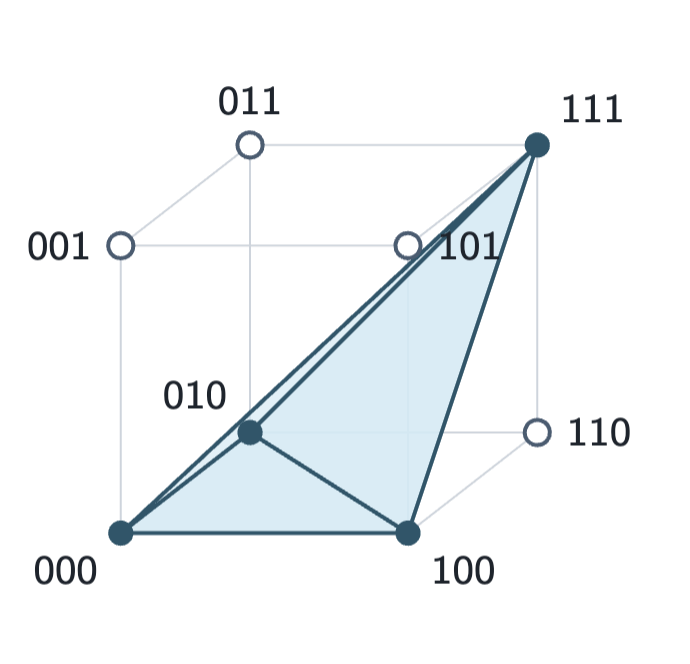
\includegraphics[width=0.5\textwidth]{figures/convex.png}
\end{figure}
从直觉来看，我们把边缘的点连成凸多边形就能变成凸包，因为把所有点都包住了，也就是说边界都是像图中的直线

那我们毕竟也不是数学系，这个就不证明了

凸多边形在高维叫多胞体，可以通过有限个线性不等式和等式来描述，这种表示方法就称为H表示

可以写成
\[
P=\{x\in\mathbb R^8\mid Ax+b\ge0,\ Cx+d=0\}.
\]

其中$A$和$b$分别表示不等式的系数矩阵和常数向量，$C$和$d$则表示等式的系数矩阵和常数向量。

因此，我们只需要将这些系数整理成矩阵形式，就可以得到完整的凸包模型：
\begin{equation}
\begin{aligned}
\min\quad &0\\
\text{s.t.}\quad
&Ax+b\ge0,\\
&Cx+d=0,\\
&x\in\{0,1\}^8.
\end{aligned}
\label{eq:lab4-full-hull-model}
\end{equation}


\paragraph{正确性分析}

首先，对于任意可达点$x\in V$，根据凸包的定义，显然有$x\in P$,所以不会漏点

不过这里有一个问题：凸包中除了原来的可达点，还会包含这些点之间的连续区域，那会不会引入新的点呢

假设存在$x\in P$，$V=\{v^{(1)},v^{(2)},...\}$

那么根据凸包的定义，存在一组非负实数$\theta_i$，使得
\[
x=\sum_{i=1}^{N}\theta_i v^{(i)},
\qquad
\theta_i\ge0,\quad
\sum_{i=1}^{N}\theta_i=1.
\]

由于$x$和$v^{(i)}$的每个坐标都只能取0或1

如果$x_j=0$，那么
\[
0=\sum_{i=1}^{N}\theta_i v_j^{(i)}.
\]

由于每一项都非负，所以对所有$\theta_i>0$的项，必有$v_j^{(i)}=0$

同理，如果$x_j=1$，那么
\[
1=\sum_{i=1}^{N}\theta_i v_j^{(i)}.
\]

因为所有$v_j^{(i)}\le1$，而$\theta_i$非负且和为1，所以对所有$\theta_i>0$的项，必有$v_j^{(i)}=1$

因此任取一个$\theta_i>0$的项，均有$x=v^{(i)}$

因此，$x$本身必然就是$V$中的某个点，不会产生新的点

综上，
\[
P\cap\{0,1\}^{8}=V.
\]

也就是说$\text{conv}(V)\cap\{0,1\}^{8}=V$

正是这个性质才让我们把$(a,b)$编码成bit,因为你如果是单纯的整数的话，就没有这么好的性质了
\paragraph{基于不可达点覆盖的贪心筛选}

那我们的H表示可能依旧得到很多不等式，我们也需要合并化简

这里我们可以采用贪心算法

假设凸包的H表示为
\[
Ax+b\ge0,\qquad Cx+d=0.
\]

对于其中第$i$条不等式，我们记为
\[
A_i x+b_i\ge0,
\]

如果某个不可达点$q\in Q$满足
\[
A_iq+b_i<0,
\]

因此，我们可以把第$i$条不等式能够排除的全部不可达点记为
\[
R_i=\{q\in Q\mid A_iq+b_i<0\}.
\]

这样，每条不等式都对应一个不可达点集合

而我们希望从这些集合中选出尽可能少的几个，使它们能够覆盖全部不可达点，那就只需要这么几个不等式就够了

这实际上就是一个集合覆盖问题。

不过需要注意，H表示中除了不等式，还可能包含等式

由于等式约束需要保留，因此那些已经违反等式的不可达点，就没有必要再通过不等式排除

我们可以先将满足
\[
Cq+d\ne0
\]
的不可达点从$Q$中删除。

剩下的不可达点记为
\[
Q_{\mathrm{remaining}}.
\]

接下来，我们每次从尚未选中的不等式中，找出能够排除最多剩余不可达点的那一条。

具体来说，选择
\[
i^*=\underset{i\in\mathrm{pool}}{\operatorname{arg\,max}}
\left|R_i\cap Q_{\mathrm{remaining}}\right|.
\]

其中$\mathrm{pool}$表示尚未选中的候选不等式集合。

选中后，将这条不等式加入保留集合，并更新剩余点集：
\[
Q_{\mathrm{remaining}}
\leftarrow
Q_{\mathrm{remaining}}\setminus R_{i^*}.
\]

然后继续寻找下一条能够排除最多剩余不可达点的不等式。

不断重复这个过程，直到
\[
Q_{\mathrm{remaining}}=\varnothing.
\]

这就说明，所有不可达点都已经被选中的约束排除了

在具体代码实现中，我们可以使用三个列表：

\begin{itemize}
    \item \texttt{remaining}：保存尚未排除的不可达点；
    \item \texttt{pool}：保存尚未选中的候选不等式；
    \item \texttt{chosen}：保存已经选中的不等式。
\end{itemize}

每次从\texttt{pool}中选择能够排除最多剩余点的不等式，将其加入\texttt{chosen}，同时从\texttt{remaining}中删除被它排除的点。

\paragraph{约简模型的正确性分析}

假设经过贪心筛选后，我们得到了保留下来的不等式集合

将这些不等式对应的系数重新组成矩阵$A'$和向量$b'$，那么约简后的模型可以写成
\begin{equation}
\begin{aligned}
\min\quad &0\\
\text{s.t.}\quad
&A'x+b'\ge0,\\
&Cx+d=0,\\
&x\in\{0,1\}^{8}.
\end{aligned}
\label{eq:lab4-reduced-hull-model}
\end{equation}

接下来，我们证明约简后的模型仍然成立

首先，所有保留下来的约束都来自原来的完整H表示

由于所有可达点都满足完整H表示，那么删除其中一部分不等式之后，可达点自然仍然满足剩下的约束

反过来，对于任意不可达点$q\in Q$，我们分两种情况讨论

如果$q$不满足等式约束
\[
Cq+d=0,
\]
那么它已经被等式排除，不可能成为模型的可行解

如果$q$满足全部等式约束，那么它就属于贪心算法初始时尚未排除的点集

由于贪心算法只有在所有剩余不可达点都被排除之后才会结束，因此必然存在某条被保留的不等式，使得
\[
A'_iq+b'_i<0.
\]

所以$q$同样不满足约简后的模型。

这说明全部不可达点都被排除

当然贪心算法求出来的不一定是最优解，不过我们也实现了减少约束数量的目的

最后，对于差分传播和线性传播，我们分别利用DDT和LAT中的非零位置构造可达点集，再独立计算凸包并进行约束筛选


\subsection{全解枚举与等价性验证}

模型建立后将目标函数设为常数$0$，仅枚举满足约束的全部二进制解，不按概率或相关度大小筛选。Gurobi的\texttt{PoolSearchMode=2}用于系统搜索多个解，\texttt{PoolSolutions}指定希望收集的解数。原始变量只有八位，取值空间为$\{0,1\}^{8}$；

对于上述四种模型，one-hot的选择变量由可达点唯一确定，其余模型不含辅助变量，因此模型的不同完整解也不超过原始八位点的取值总数。将解池容量设为严格大于这一上界，并在求解以\texttt{OPTIMAL}状态结束且解池未满时，才确认全部解已收集。

读取解池时，逐个设置\texttt{SolutionNumber}，再获取该解中各原始变量的值。

讲义使用\texttt{Xn}属性，新版本Gurobi也提供\texttt{PoolNX}属性。对one-hot模型，还应核对恰有一个选择变量取$1$，且该选择变量对应的点与原始八位变量相同。

记枚举结果在原始变量上的投影集合为$S_{\mathrm{enum}}$，则分别计算
\[
V\setminus S_{\mathrm{enum}},
\qquad
S_{\mathrm{enum}}\setminus V.
\]
前者表示漏掉的合法点，后者表示多出的非法点。只有枚举已经完成且两个差集均为空，才说明模型的二进制解恰好为$V$。差分与线性两类点集需要分别进行验证；解数相同只是必要条件，还需逐点比较。实际约束系数、条数、枚举结果及求解状态在实验内容部分记录。
